\section{Risultati}
Di seguito verranno riportati i risultati delle varie sperimentazioni con le diverse metriche descritte nel paragrafo \ref{metriche}, oltre ai tempi di elaborazioni delle esecuzioni.
\subsection{Elsevier}
\subsubsection{ALEPH}
\begin{table}[H]
\pgfplotstabletypeset[
col sep=comma,
string type,
every head row/.style={%
	before row={\toprule\addlinespace
%		\multicolumn{10}{c}{ALEPH}\\
	},
	after row=\addlinespace\midrule\addlinespace
},
every last row/.style={after row=\addlinespace\bottomrule},
columns/FOLD/.style={column name=FOLD, column type=c},
columns/TP/.style={column name=TP, column type=c},
columns/TN/.style={column name=TN, column type=c},
columns/FP/.style={column name=FP, column type=c},
columns/FN/.style={column name=FN, column type=c},
columns/precision/.style={column name=precision, column type=c},
columns/recall/.style={column name=recall, column type=c},
columns/F-Measure/.style={column name=F-Measure, column type=c},
columns/Acc/.style={column name=Accuracy, column type=c},
columns/Err/.style={column name=Error, column type=c},
]{csv/elsevier/aleph.csv}
\caption[Risultati ALEPH-Elsevier]{Risultati ottenuti con il sistema ALEPH sul dataset Elsevier}
\label{tab:ris:aleph:elsevier}
\end{table}

\begin{verbatim}
elsevier started at 14:26:44
---Fold 0 ended in: 0:00:52.449957
---Fold 1 ended in: 0:00:47.801979
---Fold 2 ended in: 0:00:53.837908
---Fold 3 ended in: 0:00:44.939273
---Fold 4 ended in: 0:00:43.786115
---Fold 5 ended in: 0:00:45.716145
---Fold 6 ended in: 0:00:53.419959
---Fold 7 ended in: 0:00:54.466414
---Fold 8 ended in: 0:00:45.072803
---Fold 9 ended in: 0:00:44.471514
elsevier ended in 0:08:05.962708
\end{verbatim}

\subsubsection{Prolog}
\begin{table}[H]
\pgfplotstabletypeset[
col sep=comma,
string type,
every head row/.style={%
	before row={\toprule\addlinespace
%		\multicolumn{10}{c}{Prolog}\\
	},
	after row=\addlinespace\midrule\addlinespace
},
every last row/.style={after row=\addlinespace\bottomrule},
columns/FOLD/.style={column name=FOLD, column type=c},
columns/TP/.style={column name=TP, column type=c},
columns/TN/.style={column name=TN, column type=c},
columns/FP/.style={column name=FP, column type=c},
columns/FN/.style={column name=FN, column type=c},
columns/precision/.style={column name=precision, column type=c},
columns/recall/.style={column name=recall, column type=c},
columns/F-Measure/.style={column name=F-Measure, column type=c},
columns/Acc/.style={column name=Accuracy, column type=c},
columns/Err/.style={column name=Error, column type=c},
]{csv/elsevier/progol.csv}
\caption[Risultati Progol-Elsevier]{Risultati ottenuti con il sistema Progol sul dataset Elsevier}
\label{tab:ris:progol:elsevier}
\end{table}

\begin{verbatim}
elsevier started at 09:22:02
---Fold 0 ended in: 0:00:38.425921
---Fold 1 ended in: 0:00:40.896260
---Fold 2 ended in: 0:00:47.197656
---Fold 3 ended in: 0:01:24.320783
---Fold 4 ended in: 0:00:45.006192
---Fold 5 ended in: 0:00:43.862157
---Fold 6 ended in: 0:00:33.893715
---Fold 7 ended in: 0:00:46.741183
---Fold 8 ended in: 0:00:42.525816
---Fold 9 ended in: 0:00:39.602502
elsevier ended in 0:07:42.472820
\end{verbatim}


\subsubsection{FOIL}
\begin{table}[H]
\pgfplotstabletypeset[
col sep=comma,
string type,
every head row/.style={%
	before row={\toprule\addlinespace
%		\multicolumn{10}{c}{FOIL}\\
	},
	after row=\addlinespace\midrule\addlinespace
},
every last row/.style={after row=\addlinespace\bottomrule},
columns/FOLD/.style={column name=FOLD, column type=c},
columns/TP/.style={column name=TP, column type=c},
columns/TN/.style={column name=TN, column type=c},
columns/FP/.style={column name=FP, column type=c},
columns/FN/.style={column name=FN, column type=c},
columns/precision/.style={column name=precision, column type=c},
columns/recall/.style={column name=recall, column type=c},
columns/F-Measure/.style={column name=F-Measure, column type=c},
columns/Acc/.style={column name=Accuracy, column type=c},
columns/Err/.style={column name=Error, column type=c},
]{csv/elsevier/foil.csv}
\caption[Risultati FOIL-Elsevier]{Risultati ottenuti con il sistema FOIL sul dataset Elsevier}
\label{tab:ris:foil:elsevier}
\end{table}

\begin{verbatim}
elsevier started at 09:11:46
---Fold 0 ended in: 0:00:03.258203
---Fold 1 ended in: 0:00:02.868314
---Fold 2 ended in: 0:00:02.853725
---Fold 3 ended in: 0:00:03.356398
---Fold 4 ended in: 0:00:03.351272
---Fold 5 ended in: 0:00:02.746340
---Fold 6 ended in: 0:00:01.770807
---Fold 7 ended in: 0:00:02.997800
---Fold 8 ended in: 0:00:12.297267
---Fold 9 ended in: 0:00:01.600430
elsevier ended in 0:00:37.101084
\end{verbatim}

\subsubsection{Grafici}
\paragraph{Precision}
\begin{figure}[H]
	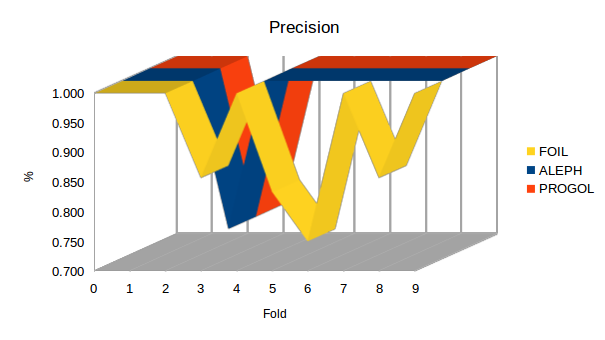
\includegraphics[width=1.1\textwidth]{img/datasetGraph/elsevier/precision.png}
	\label{Elsevier-Precision}
\end{figure}

\paragraph{Recall}
\begin{figure}[H]
	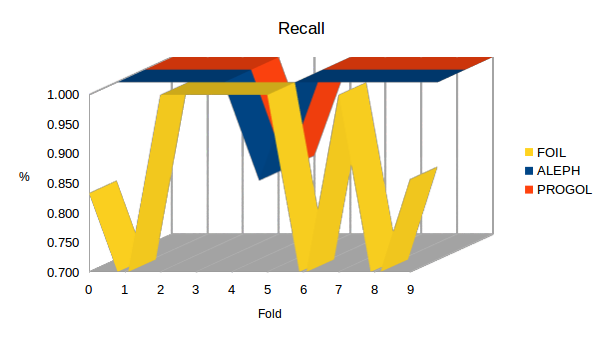
\includegraphics[width=1.1\textwidth]{img/datasetGraph/elsevier/recall.png}
	\label{Elsevier-Recall}
\end{figure}

\paragraph{F-Measure}
\begin{figure}[H]
	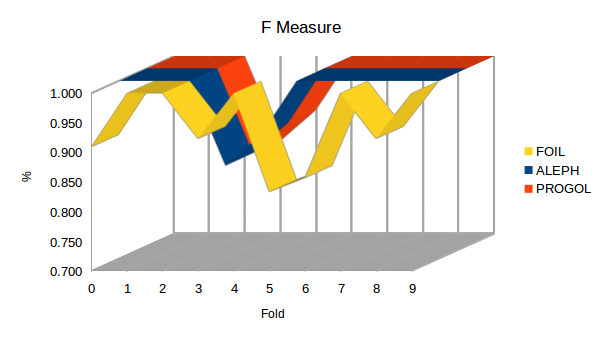
\includegraphics[width=1.1\textwidth]{img/datasetGraph/elsevier/fm.png}
	\label{Elsevier-F-measure}
\end{figure}

\paragraph{Accuracy}
\begin{figure}[H]
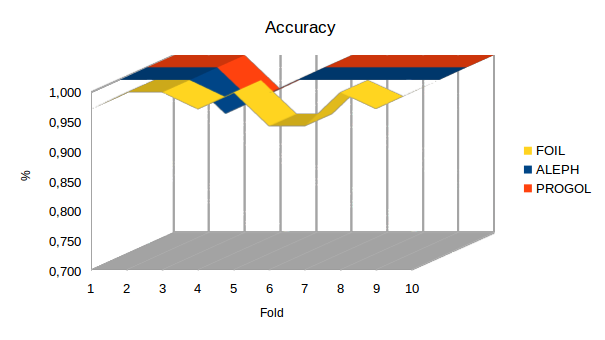
\includegraphics[width=1.1\textwidth]{img/datasetGraph/elsevier/accuracy.png}
\label{Elsevier-Accuracy}
\end{figure}

\paragraph{Error}
\begin{figure}[H]
	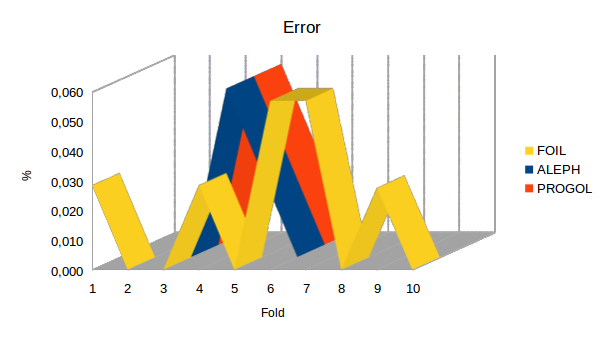
\includegraphics[width=1.1\textwidth]{img/datasetGraph/elsevier/error.png}
	\label{Elsevier-Error}
\end{figure}

\subsection{JMLR}
\subsubsection{ALEPH}
\begin{table}[H]
\pgfplotstabletypeset[
col sep=comma,
string type,
every head row/.style={%
	before row={\toprule\addlinespace
		%		\multicolumn{10}{c}{ALEPH}\\
	},
	after row=\addlinespace\midrule\addlinespace
},
every last row/.style={after row=\addlinespace\bottomrule},
columns/FOLD/.style={column name=FOLD, column type=c},
columns/TP/.style={column name=TP, column type=c},
columns/TN/.style={column name=TN, column type=c},
columns/FP/.style={column name=FP, column type=c},
columns/FN/.style={column name=FN, column type=c},
columns/precision/.style={column name=precision, column type=c},
columns/recall/.style={column name=recall, column type=c},
columns/F-Measure/.style={column name=F-Measure, column type=c},
columns/Acc/.style={column name=Accuracy, column type=c},
columns/Err/.style={column name=Error, column type=c},
]{csv/jmlr/aleph.csv}
\caption[Risultati ALEPH-JMLR]{Risultati ottenuti con il sistema ALEPH sul dataset JMLR}
\label{tab:ris:aleph:jmlr}
\end{table}

\begin{verbatim}
jmlr started at 14:34:50
---Fold 0 ended in: 0:00:44.040336
---Fold 1 ended in: 0:00:58.375317
---Fold 2 ended in: 0:00:40.177290
---Fold 3 ended in: 0:00:31.072195
---Fold 4 ended in: 0:00:57.077835
---Fold 5 ended in: 0:00:58.648341
---Fold 6 ended in: 0:00:58.353248
---Fold 7 ended in: 0:00:58.888839
---Fold 8 ended in: 0:00:42.341782
---Fold 9 ended in: 0:00:43.150318
jmlr ended in 0:08:12.126228
\end{verbatim}


\subsubsection{Prolog}
\begin{table}[H]
\pgfplotstabletypeset[
col sep=comma,
string type,
every head row/.style={%
	before row={\toprule\addlinespace
		%		\multicolumn{10}{c}{Prolog}\\
	},
	after row=\addlinespace\midrule\addlinespace
},
every last row/.style={after row=\addlinespace\bottomrule},
columns/FOLD/.style={column name=FOLD, column type=c},
columns/TP/.style={column name=TP, column type=c},
columns/TN/.style={column name=TN, column type=c},
columns/FP/.style={column name=FP, column type=c},
columns/FN/.style={column name=FN, column type=c},
columns/precision/.style={column name=precision, column type=c},
columns/recall/.style={column name=recall, column type=c},
columns/F-Measure/.style={column name=F-Measure, column type=c},
columns/Acc/.style={column name=Accuracy, column type=c},
columns/Err/.style={column name=Error, column type=c},
]{csv/jmlr/progol.csv}
\caption[Risultati ]{Risultati ottenuti con il sistema Progol sul dataset JMLR}
\label{tab:ris:progol:jmlr}
\end{table}

\begin{verbatim}
jmlr started at 09:29:44
---Fold 0 ended in: 0:00:26.084275
---Fold 1 ended in: 0:00:45.996500
---Fold 2 ended in: 0:00:37.654357
---Fold 3 ended in: 0:00:29.765864
---Fold 4 ended in: 0:00:41.809093
---Fold 5 ended in: 0:00:37.723421
---Fold 6 ended in: 0:00:19.029631
---Fold 7 ended in: 0:00:49.946552
---Fold 8 ended in: 0:00:34.581277
---Fold 9 ended in: 0:00:34.694070
jmlr ended in 0:05:57.285763
\end{verbatim}

\subsubsection{FOIL}
\begin{table}[H]
\pgfplotstabletypeset[
col sep=comma,
string type,
every head row/.style={%
	before row={\toprule\addlinespace
		%		\multicolumn{10}{c}{FOIL}\\
	},
	after row=\addlinespace\midrule\addlinespace
},
every last row/.style={after row=\addlinespace\bottomrule},
columns/FOLD/.style={column name=FOLD, column type=c},
columns/TP/.style={column name=TP, column type=c},
columns/TN/.style={column name=TN, column type=c},
columns/FP/.style={column name=FP, column type=c},
columns/FN/.style={column name=FN, column type=c},
columns/precision/.style={column name=precision, column type=c},
columns/recall/.style={column name=recall, column type=c},
columns/F-Measure/.style={column name=F-Measure, column type=c},
columns/Acc/.style={column name=Accuracy, column type=c},
columns/Err/.style={column name=Error, column type=c},
]{csv/jmlr/foil.csv}
\caption[Risultati FOIL-JMLR]{Risultati ottenuti con il sistema FOIL sul dataset JMLR}
\label{tab:ris:foil:jmlr}
\end{table}

\begin{verbatim}
jmlr started at 09:12:23
---Fold 0 ended in: 0:00:02.759541
---Fold 1 ended in: 0:00:05.639292
---Fold 2 ended in: 0:00:07.404179
---Fold 3 ended in: 0:00:03.042006
---Fold 4 ended in: 0:00:05.479597
---Fold 5 ended in: 0:00:03.189191
---Fold 6 ended in: 0:00:02.824482
---Fold 7 ended in: 0:00:02.231835
---Fold 8 ended in: 0:00:03.894108
---Fold 9 ended in: 0:00:03.966871
jmlr ended in 0:00:40.431931
\end{verbatim}


\subsubsection{Grafici}
\paragraph{Precision}
\begin{figure}[H]
	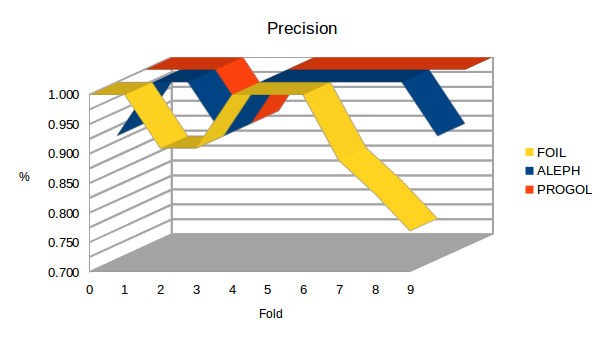
\includegraphics[width=1.1\textwidth]{img/datasetGraph/jmlr/precision.png}
	\label{JMLR-Precision}
\end{figure}

\paragraph{Recall}
\begin{figure}[H]
	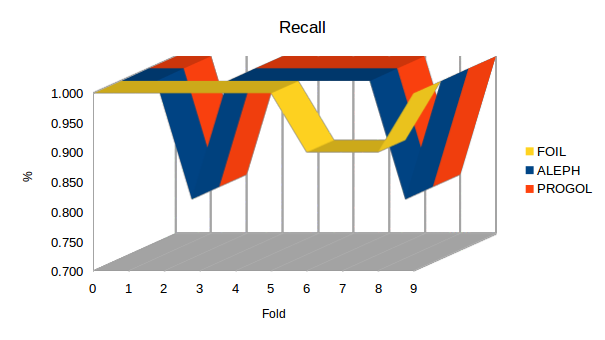
\includegraphics[width=1.1\textwidth]{img/datasetGraph/jmlr/recall.png}
	\label{JMLR-Recall}
\end{figure}

\paragraph{F-Measure}
\begin{figure}[H]
	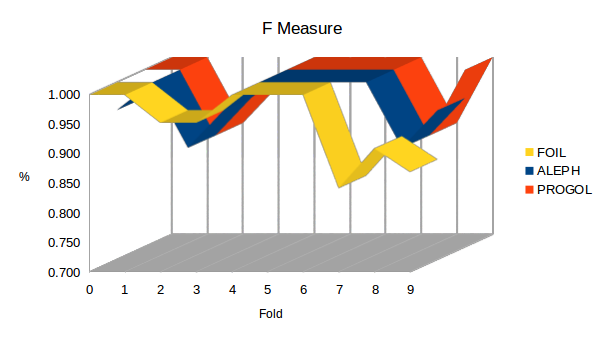
\includegraphics[width=1.1\textwidth]{img/datasetGraph/jmlr/fm.png}
	\label{JMLR-F-measure}
\end{figure}

\paragraph{Accuracy}
\begin{figure}[H]
	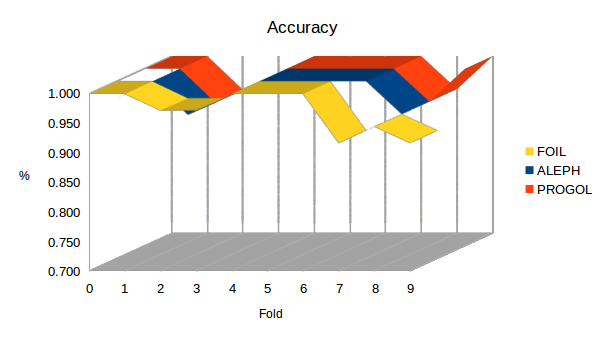
\includegraphics[width=1.1\textwidth]{img/datasetGraph/jmlr/accuracy.png}
	\label{JMLR-Accuracy}
\end{figure}

\paragraph{Error}
\begin{figure}[H]
	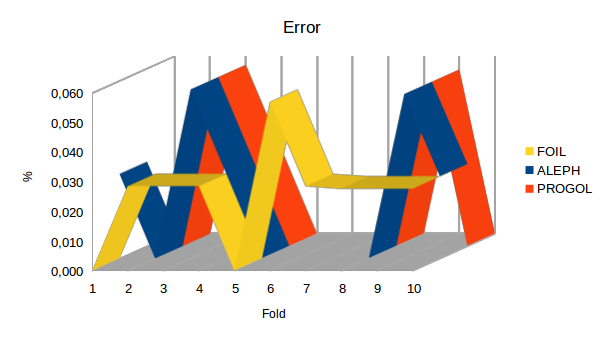
\includegraphics[width=1.1\textwidth]{img/datasetGraph/jmlr/error.png}
	\label{JMLR-Error}
\end{figure}


\subsection{SVLN}
\subsubsection{ALEPH}
\begin{table}[H]
\pgfplotstabletypeset[
col sep=comma,
string type,
every head row/.style={%
	before row={\toprule\addlinespace
		%		\multicolumn{10}{c}{ALEPH}\\
	},
	after row=\addlinespace\midrule\addlinespace
},
every last row/.style={after row=\addlinespace\bottomrule},
columns/FOLD/.style={column name=FOLD, column type=c},
columns/TP/.style={column name=TP, column type=c},
columns/TN/.style={column name=TN, column type=c},
columns/FP/.style={column name=FP, column type=c},
columns/FN/.style={column name=FN, column type=c},
columns/precision/.style={column name=precision, column type=c},
columns/recall/.style={column name=recall, column type=c},
columns/F-Measure/.style={column name=F-Measure, column type=c},
columns/Acc/.style={column name=Accuracy, column type=c},
columns/Err/.style={column name=Error, column type=c},
]{csv/svln/aleph.csv}
\caption[Risultati ALEPH-SVLN]{Risultati ottenuti con il sistema ALEPH sul dataset JMLR}
\label{tab:ris:aleph:svln}
\end{table}

\begin{verbatim}
svln started at 18:53:32
---Fold 0 ended in: 0:01:54.234807
---Fold 1 ended in: 0:01:35.397646
---Fold 2 ended in: 0:01:43.559253
---Fold 3 ended in: 0:01:52.177093
---Fold 4 ended in: 0:02:31.127063
---Fold 5 ended in: 0:01:47.824715
---Fold 6 ended in: 0:01:40.269009
---Fold 7 ended in: 0:01:15.299631
---Fold 8 ended in: 0:01:39.995804
---Fold 9 ended in: 0:02:01.367264
svln ended in 0:18:01.252851
\end{verbatim}


\subsubsection{Progol}
\begin{table}[H]
\pgfplotstabletypeset[
col sep=comma,
string type,
every head row/.style={%
	before row={\toprule\addlinespace
		%		\multicolumn{10}{c}{Prolog}\\
	},
	after row=\addlinespace\midrule\addlinespace
},
every last row/.style={after row=\addlinespace\bottomrule},
columns/FOLD/.style={column name=FOLD, column type=c},
columns/TP/.style={column name=TP, column type=c},
columns/TN/.style={column name=TN, column type=c},
columns/FP/.style={column name=FP, column type=c},
columns/FN/.style={column name=FN, column type=c},
columns/precision/.style={column name=precision, column type=c},
columns/recall/.style={column name=recall, column type=c},
columns/F-Measure/.style={column name=F-Measure, column type=c},
columns/Acc/.style={column name=Accuracy, column type=c},
columns/Err/.style={column name=Error, column type=c},
]{csv/svln/progol.csv}
\caption[Risultati Progol-SVLN]{Risultati ottenuti con il sistema Progol sul dataset SVLN}
\label{tab:ris}
\end{table}

\begin{verbatim}
svln started at 12:43:51
---Fold 0 ended in: 0:01:04.320244
---Fold 1 ended in: 0:01:24.453421
---Fold 2 ended in: 0:01:12.648375
---Fold 3 ended in: 0:01:00.633611
---Fold 4 ended in: 0:01:18.982588
---Fold 5 ended in: 0:01:16.183743
---Fold 6 ended in: 0:01:00.154165
---Fold 7 ended in: 0:00:42.924736
---Fold 8 ended in: 0:01:24.184806
---Fold 9 ended in: 0:01:44.461413
svln ended in 0:12:08.991536
\end{verbatim}

\subsubsection{FOIL}
\begin{table}[H]
\pgfplotstabletypeset[
col sep=comma,
string type,
every head row/.style={%
	before row={\toprule\addlinespace
		%		\multicolumn{10}{c}{FOIL}\\
	},
	after row=\addlinespace\midrule\addlinespace
},
every last row/.style={after row=\addlinespace\bottomrule},
columns/FOLD/.style={column name=FOLD, column type=c},
columns/TP/.style={column name=TP, column type=c},
columns/TN/.style={column name=TN, column type=c},
columns/FP/.style={column name=FP, column type=c},
columns/FN/.style={column name=FN, column type=c},
columns/precision/.style={column name=precision, column type=c},
columns/recall/.style={column name=recall, column type=c},
columns/F-Measure/.style={column name=F-Measure, column type=c},
columns/Acc/.style={column name=Accuracy, column type=c},
columns/Err/.style={column name=Error, column type=c},
]{csv/svln/foil.csv}
\caption[Risultati FOIL-SVLN]{Risultati ottenuti con il sistema FOIL sul dataset SVLN}
\label{tab:ris:foil:svln}
\end{table}

\begin{verbatim}
svln started at 09:13:04
---Fold 0 ended in: 0:00:00.328284
---Fold 1 ended in: 0:00:00.238981
---Fold 2 ended in: 0:00:00.294530
---Fold 3 ended in: 0:00:00.207063
---Fold 4 ended in: 0:00:00.242937
---Fold 5 ended in: 0:00:00.191957
---Fold 6 ended in: 0:00:00.194648
---Fold 7 ended in: 0:00:00.340427
---Fold 8 ended in: 0:00:00.318204
---Fold 9 ended in: 0:00:00.208281
svln ended in 0:00:02.566150
\end{verbatim}

\subsubsection{Grafici}
\paragraph{Precision}
\begin{figure}[H]
	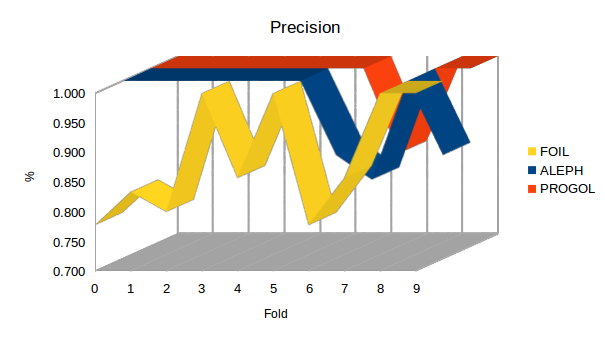
\includegraphics[width=1.1\textwidth]{img/datasetGraph/svln/precision.png}
	\label{svln-Precision}
\end{figure}
\paragraph{Recall}
\begin{figure}[H]
	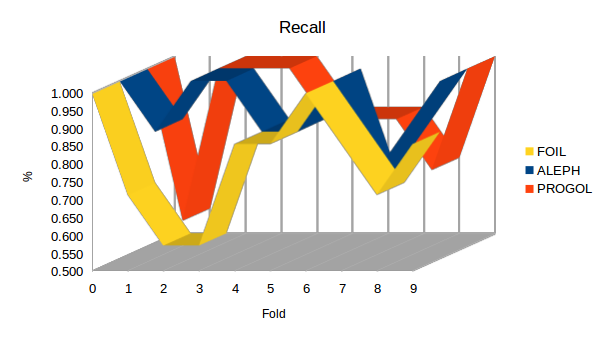
\includegraphics[width=1.1\textwidth]{img/datasetGraph/svln/recall.png}
	\label{svln-Recall}
\end{figure}
\paragraph{F-Measure}
\begin{figure}[H]
	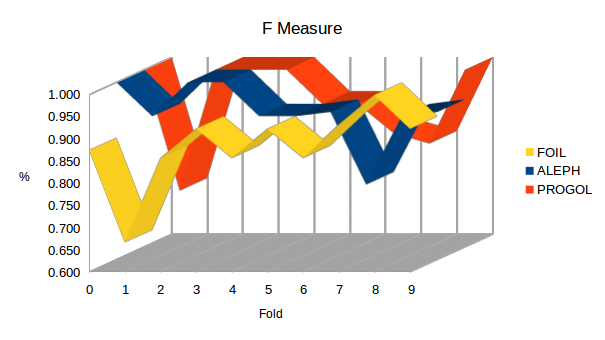
\includegraphics[width=1.1\textwidth]{img/datasetGraph/svln/fm.png}
	\label{svln-F-measure}
\end{figure}
\paragraph{Accuracy}
\begin{figure}[H]
	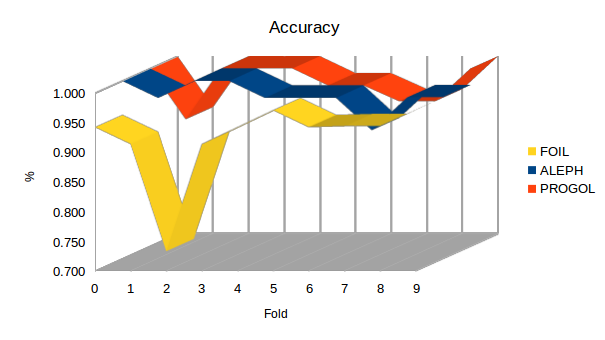
\includegraphics[width=1.1\textwidth]{img/datasetGraph/svln/accuracy.png}
	\label{svln-Accuracy}
\end{figure}
\paragraph{Error}
\begin{figure}[H]
	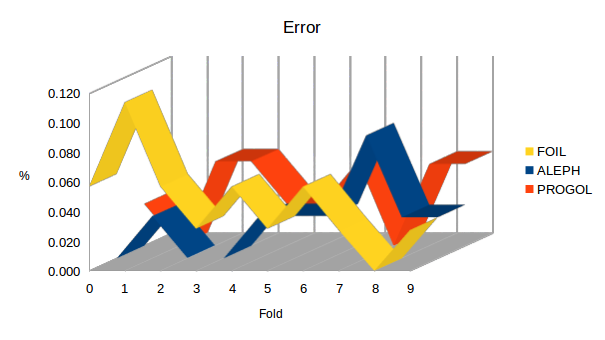
\includegraphics[width=1.1\textwidth]{img/datasetGraph/svln/error.png}
	\label{svln-Error}
\end{figure}

\subsection{MLJ - discretizzato}
\subsubsection{ALEPH}
\begin{table}[H]
\pgfplotstabletypeset[
col sep=comma,
string type,
every head row/.style={%
	before row={\toprule\addlinespace
		%		\multicolumn{10}{c}{ALEPH}\\
	},
	after row=\addlinespace\midrule\addlinespace
},
every last row/.style={after row=\addlinespace\bottomrule},
columns/FOLD/.style={column name=FOLD, column type=c},
columns/TP/.style={column name=TP, column type=c},
columns/TN/.style={column name=TN, column type=c},
columns/FP/.style={column name=FP, column type=c},
columns/FN/.style={column name=FN, column type=c},
columns/precision/.style={column name=precision, column type=c},
columns/recall/.style={column name=recall, column type=c},
columns/F-Measure/.style={column name=F-Measure, column type=c},
columns/Acc/.style={column name=Accuracy, column type=c},
columns/Err/.style={column name=Error, column type=c},
]{csv/mlj/discr/aleph.csv}
\caption[Risultati ALEPH-MLJ Discretizzato]{Risultati ottenuti con il sistema ALEPH sul dataset MLJ discretizzato}
\label{tab:ris:aleph:mlj:discr}
\end{table}

\begin{verbatim}
mlj discr started at 12:38:52
---Fold 0 ended in: 0:06:32.987887
---Fold 1 ended in: 0:06:55.407367
---Fold 2 ended in: 0:06:38.581722
---Fold 3 ended in: 0:06:40.096561
---Fold 4 ended in: 0:06:42.671273
---Fold 5 ended in: 0:06:46.315155
---Fold 6 ended in: 0:06:29.094981
---Fold 7 ended in: 0:06:49.495072
---Fold 8 ended in: 0:05:32.322452
---Fold 9 ended in: 0:05:26.615672
mlj discr ended in 1:04:33.588808
\end{verbatim}

\subsubsection{Prolog}
\begin{table}[H]
\pgfplotstabletypeset[
col sep=comma,
string type,
every head row/.style={%
	before row={\toprule\addlinespace
		%		\multicolumn{10}{c}{Prolog}\\
	},
	after row=\addlinespace\midrule\addlinespace
},
every last row/.style={after row=\addlinespace\bottomrule},
columns/FOLD/.style={column name=FOLD, column type=c},
columns/TP/.style={column name=TP, column type=c},
columns/TN/.style={column name=TN, column type=c},
columns/FP/.style={column name=FP, column type=c},
columns/FN/.style={column name=FN, column type=c},
columns/precision/.style={column name=precision, column type=c},
columns/recall/.style={column name=recall, column type=c},
columns/F-Measure/.style={column name=F-Measure, column type=c},
columns/Acc/.style={column name=Accuracy, column type=c},
columns/Err/.style={column name=Error, column type=c},
]{csv/mlj/discr/progol.csv}
\caption[Risultati Progol-MLJ Discretizzato]{Risultati ottenuti con il sistema Progol sul dataset MLJ discretizzato.}
\label{tab:ris:progol:mlj:discr}
\end{table}

\begin{verbatim}
mlj discr started at 14:35:28
---Fold 0 ended in: 0:05:33.172855
---Fold 1 ended in: 0:04:24.460047
---Fold 2 ended in: 0:06:21.096485
---Fold 3 ended in: 0:04:39.550606
---Fold 4 ended in: 0:05:39.287544
---Fold 5 ended in: 0:04:42.005965
---Fold 6 ended in: 0:05:36.268812
---Fold 7 ended in: 0:05:15.292060
---Fold 8 ended in: 0:04:34.640609
---Fold 9 ended in: 0:04:57.705908
mlj discr ended in 0:51:43.481549
\end{verbatim}


\subsubsection{FOIL}
\begin{table}[H]
\pgfplotstabletypeset[
col sep=comma,
string type,
every head row/.style={%
	before row={\toprule\addlinespace
		%		\multicolumn{10}{c}{FOIL}\\
	},
	after row=\addlinespace\midrule\addlinespace
},
every last row/.style={after row=\addlinespace\bottomrule},
columns/FOLD/.style={column name=FOLD, column type=c},
columns/TP/.style={column name=TP, column type=c},
columns/TN/.style={column name=TN, column type=c},
columns/FP/.style={column name=FP, column type=c},
columns/FN/.style={column name=FN, column type=c},
columns/precision/.style={column name=precision, column type=c},
columns/recall/.style={column name=recall, column type=c},
columns/F-Measure/.style={column name=F-Measure, column type=c},
columns/Acc/.style={column name=Accuracy, column type=c},
columns/Err/.style={column name=Error, column type=c},
]{csv/mlj/discr/foil.csv}
\caption[Risultati FOIL-MLJ discretizzato]{Risultati ottenuti con il sistema FOIL sul dataset MLJ discretizzato}
\label{tab:ris:foil:mlj:discr}
\end{table}

\begin{verbatim}
mlj discr started at 11:59:39
---Fold 0 ended in: 0:00:00.224591
---Fold 1 ended in: 0:00:00.237705
---Fold 2 ended in: 0:00:00.231943
---Fold 3 ended in: 0:00:00.225304
---Fold 4 ended in: 0:00:00.269991
---Fold 5 ended in: 0:00:00.227715
---Fold 6 ended in: 0:00:00.215050
---Fold 7 ended in: 0:00:00.271112
---Fold 8 ended in: 0:00:00.182183
---Fold 9 ended in: 0:00:00.206913
mlj discr ended in 0:00:02.293352
\end{verbatim}

\subsubsection{Grafici}
\paragraph{Precision}
\begin{figure}[H]
	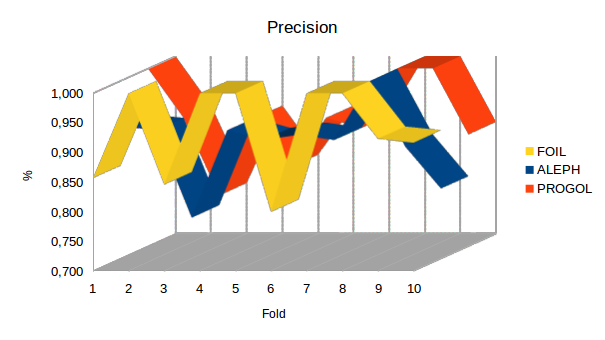
\includegraphics[width=1.1\textwidth]{img/datasetGraph/mlj/discr/precision.png}
	\label{mljdiscr-Precision}
\end{figure}
\paragraph{Recall}
\begin{figure}[H]
	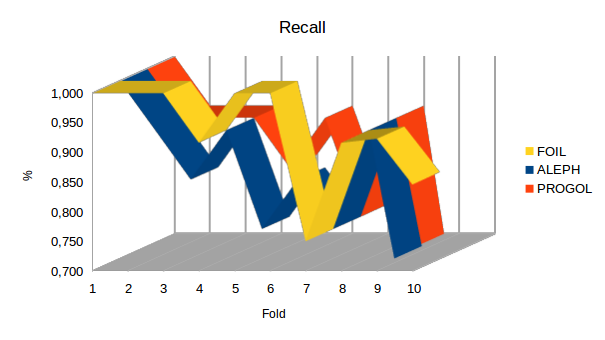
\includegraphics[width=1.1\textwidth]{img/datasetGraph/mlj/discr/recall.png}
	\label{mljdiscr-Recall}
\end{figure}
\paragraph{F-Measure}
\begin{figure}[H]
	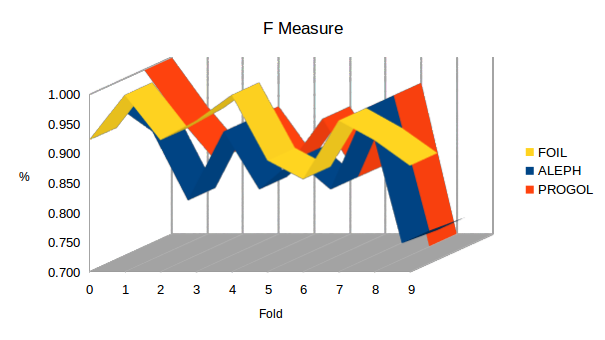
\includegraphics[width=1.1\textwidth]{img/datasetGraph/mlj/discr/fm.png}
	\label{mljdiscr-F-measure}
\end{figure}
\paragraph{Accuracy}
\begin{figure}[H]
	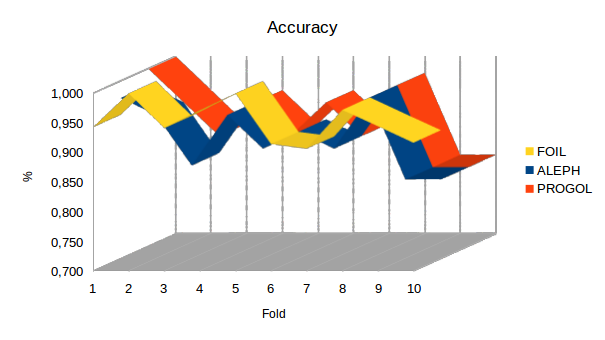
\includegraphics[width=1.1\textwidth]{img/datasetGraph/mlj/discr/accuracy.png}
	\label{mljdiscr-Accuracy}
\end{figure}
\paragraph{Error}
\begin{figure}[H]
	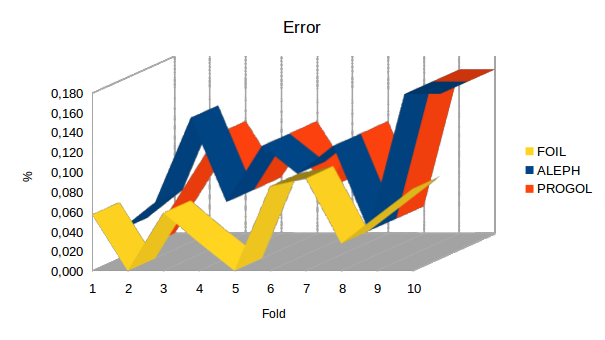
\includegraphics[width=1.1\textwidth]{img/datasetGraph/mlj/discr/error.png}
	\label{mljdiscr-Error}
\end{figure}

\subsection{MLJ - non discretizzato}
\subsubsection{ALEPH}
\begin{table}[H]
\pgfplotstabletypeset[
col sep=comma,
string type,
every head row/.style={%
	before row={\toprule\addlinespace
		%		\multicolumn{10}{c}{ALEPH}\\
	},
	after row=\addlinespace\midrule\addlinespace
},
every last row/.style={after row=\addlinespace\bottomrule},
columns/FOLD/.style={column name=FOLD, column type=c},
columns/TP/.style={column name=TP, column type=c},
columns/TN/.style={column name=TN, column type=c},
columns/FP/.style={column name=FP, column type=c},
columns/FN/.style={column name=FN, column type=c},
columns/precision/.style={column name=precision, column type=c},
columns/recall/.style={column name=recall, column type=c},
columns/F-Measure/.style={column name=F-Measure, column type=c},
columns/Acc/.style={column name=Accuracy, column type=c},
columns/Err/.style={column name=Error, column type=c},
]{csv/mlj/nodiscr/aleph.csv}
\caption[Risultati ALEPH-MLJ non discretizzato]{Risultati ottenuti con il sistema ALEPH sul dataset MLJ non discretizzato}
\label{tab:ris:aleph:mlj:nondiscr}
\end{table}

\begin{verbatim}
mlj nodiscr started at 13:57:41
---Fold 0 ended in: 0:02:21.787734
---Fold 1 ended in: 0:04:07.386826
---Fold 2 ended in: 0:04:17.316495
---Fold 3 ended in: 0:04:06.532924
---Fold 4 ended in: 0:04:10.948141
---Fold 5 ended in: 0:04:06.952672
---Fold 6 ended in: 0:04:48.798386
---Fold 7 ended in: 0:04:43.446125
---Fold 8 ended in: 0:08:46.085098
---Fold 9 ended in: 0:05:54.209124
mlj nodiscr ended in 0:47:23.464204
\end{verbatim}

\subsubsection{Prolog}
\begin{table}[H]
\pgfplotstabletypeset[
col sep=comma,
string type,
every head row/.style={%
	before row={\toprule\addlinespace
		%		\multicolumn{10}{c}{Prolog}\\
	},
	after row=\addlinespace\midrule\addlinespace
},
every last row/.style={after row=\addlinespace\bottomrule},
columns/FOLD/.style={column name=FOLD, column type=c},
columns/TP/.style={column name=TP, column type=c},
columns/TN/.style={column name=TN, column type=c},
columns/FP/.style={column name=FP, column type=c},
columns/FN/.style={column name=FN, column type=c},
columns/precision/.style={column name=precision, column type=c},
columns/recall/.style={column name=recall, column type=c},
columns/F-Measure/.style={column name=F-Measure, column type=c},
columns/Acc/.style={column name=Accuracy, column type=c},
columns/Err/.style={column name=Error, column type=c},
]{csv/mlj/nodiscr/progol.csv}
\caption[Risultati Progol-MLJ non discretizzato]{Risultati ottenuti con il sistema Progol sul dataset MLJ non discretizzato}
\label{tab:ris:progol:mlj:nodiscr}
\end{table}

\begin{verbatim}
mlj nodiscr started at 15:13:39
---Fold 0 ended in: 0:01:56.835496
---Fold 1 ended in: 0:03:59.207766
---Fold 2 ended in: 0:05:05.807433
---Fold 3 ended in: 0:06:07.573072
---Fold 4 ended in: 0:02:00.128641
---Fold 5 ended in: 0:06:00.366362
---Fold 6 ended in: 0:03:54.306654
---Fold 7 ended in: 0:04:42.558320
---Fold 8 ended in: 0:02:21.500061
---Fold 9 ended in: 0:02:10.637707
mlj nodiscr ended in 0:38:18.922015
\end{verbatim}

\subsubsection{FOIL}

\begin{table}[H]
\pgfplotstabletypeset[
col sep=comma,
string type,
every head row/.style={%
	before row={\toprule\addlinespace
		%		\multicolumn{10}{c}{FOIL}\\
	},
	after row=\addlinespace\midrule\addlinespace
},
every last row/.style={after row=\addlinespace\bottomrule},
columns/FOLD/.style={column name=FOLD, column type=c},
columns/TP/.style={column name=TP, column type=c},
columns/TN/.style={column name=TN, column type=c},
columns/FP/.style={column name=FP, column type=c},
columns/FN/.style={column name=FN, column type=c},
columns/precision/.style={column name=precision, column type=c},
columns/recall/.style={column name=recall, column type=c},
columns/F-Measure/.style={column name=F-Measure, column type=c},
columns/Acc/.style={column name=Accuracy, column type=c},
columns/Err/.style={column name=Error, column type=c}
]{csv/mlj/nodiscr/foil.csv}
\caption[Risultati FOIL-MLJ non discretizzato]{Risultati ottenuti con il sistema FOIL sul dataset MLJ non discretizzato}
\label{tab:ris:foil:mlj:nondiscr}
\end{table}

\begin{verbatim}
mlj nodiscr started at 13:48:52
---Fold 0 ended in: 0:00:02.204258
---Fold 1 ended in: 0:00:26.650516
---Fold 2 ended in: 0:00:26.171711
---Fold 3 ended in: 0:00:46.732210
---Fold 4 ended in: 0:00:51.158960
---Fold 5 ended in: 0:00:05.917821
---Fold 6 ended in: 0:00:23.688156
---Fold 7 ended in: 0:00:28.056554
---Fold 8 ended in: 0:00:51.933317
---Fold 9 ended in: 0:00:06.915890
mlj nodiscr ended in 0:04:29.430078
\end{verbatim}

\subsubsection{Grafici}
\paragraph{Precision}
\begin{figure}[H]
	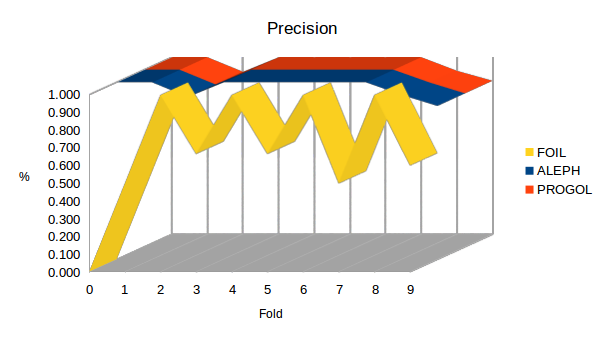
\includegraphics[width=1.1\textwidth]{img/datasetGraph/mlj/nodiscr/precision.png}
	\label{mljnodiscr-Precision}
\end{figure}
\paragraph{Recall}
\begin{figure}[H]
	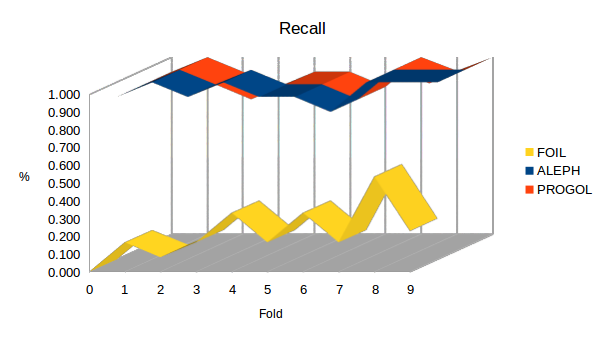
\includegraphics[width=1.1\textwidth]{img/datasetGraph/mlj/nodiscr/recall.png}
	\label{mljnodiscr-Recall}
\end{figure}
\paragraph{F-Measure}
\begin{figure}[H]
	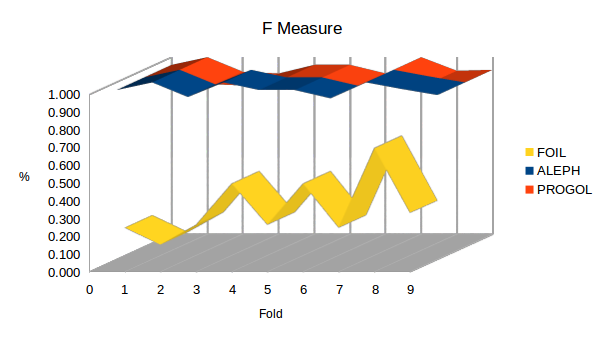
\includegraphics[width=1.1\textwidth]{img/datasetGraph/mlj/nodiscr/fm.png}
	\label{mljnodiscr-F-measure}
\end{figure}
\paragraph{Accuracy}
\begin{figure}[H]
	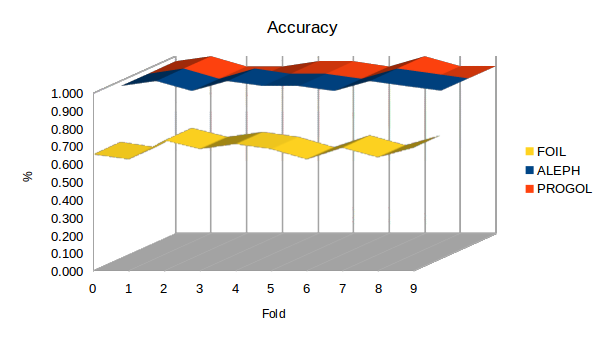
\includegraphics[width=1.1\textwidth]{img/datasetGraph/mlj/nodiscr/accuracy.png}
	\label{mljnodiscr-Accuracy}
\end{figure}
\paragraph{Error}
\begin{figure}[H]
	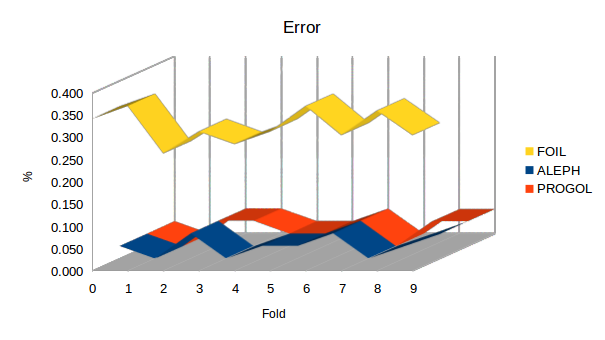
\includegraphics[width=1.1\textwidth]{img/datasetGraph/mlj/nodiscr/error.png}
	\label{mljnodiscr-Error}
\end{figure}
